\documentclass{beamer}

% Top-aligning columns within a top-aligned frame
% https://tex.stackexchange.com/questions/16447/beamer-top-aligning-columns-within-a-top-aligned-frame
\makeatletter
\newenvironment{myitemize}{%
   \setlength{\topsep}{0pt}
   \setlength{\partopsep}{0pt}
   \renewcommand*{\@listi}{\leftmargin\leftmargini \parsep\z@ \topsep\z@ \itemsep\z@}
   \let\@listI\@listi
   \itemize
}{\enditemize}
\makeatother  

\usepackage[USenglish]{babel}
\usepackage[utf8]{inputenc}
\usepackage{amssymb, amsmath}
\usepackage{bm}
\usepackage{color}
\usepackage{tikz}
\usepackage{url}

\definecolor{links}{HTML}{2A1B81}
\hypersetup{colorlinks,linkcolor=,urlcolor=links}

\usetheme{Boadilla}

\bibliographystyle{apalike}
% make bibliography entries smaller
%\renewcommand\bibfont{\scriptsize}
% Now get rid of all the colours
\setbeamercolor*{bibliography entry title}{fg=black}
\setbeamercolor*{bibliography entry author}{fg=black}
\setbeamercolor*{bibliography entry location}{fg=black}
\setbeamercolor*{bibliography entry note}{fg=black}

\newcommand{\lnorm}[1]{\left\lVert#1\right\rVert^2}
\newcommand{\norm}[1]{\left\lVert#1\right\rVert}

% and kill the abominable icon
\setbeamertemplate{bibliography item}{}

\begin{document}
\title[The Secret Sharer]{The Secret Sharer: Evaluating and Testing Unintended Memorization in Neural Networks}  
\author{Radek Bartyzal}
\date{24. 11. 2020} 
\institute{GLAMI AI}

\frame{\titlepage} 

%--------- END Frame 12 -------------
\begin{frame}{Motivation}

Paper is by Google Brain, BAIR from 2019.
\vfill

Current state:
\begin{itemize}
\item we are training large NLP models
\item scraping a lot of data
\item possibly confidential user data
\end{itemize}
\vfill
Questions:
\begin{itemize}
\item can we extract e.g. card numbers (yes)
\item is it due to overfitting? (no)
\item how to quantify it? (exposure metric)
\item Is my model likely to memorize and potentially expose rarely- occurring, sensitive sequences in training data?
\end{itemize}

\end{frame}
%--------- END Frame 12 -------------
\begin{frame}{Motivation}

\begin{figure}[h]
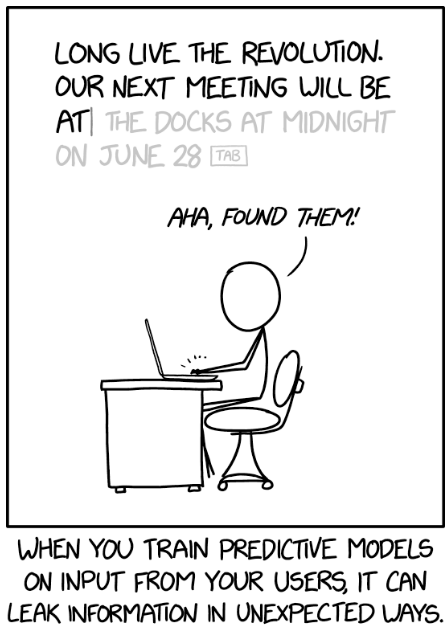
\includegraphics[width=0.4\textwidth]{img/xkcd}
\caption{There is an XKCD for everything \cite{cit:xkcd}.}
\end{figure}

\end{frame}
%--------- END Frame 12 -------------
\begin{frame}{Threat model}

Threat model:
\begin{itemize}
\item black box attack
\item 10 000s of queries
\item sees logits / probabilities of the model outputs = it's harder without this
\end{itemize}

\vfill

\begin{block}{No Transformers?}
They only test LSTMs and qRNNS not Transformers!
\end{block}

\end{frame}
%--------- END Frame 12 -------------
\begin{frame}{Methodics}

Is my model likely to memorize and potentially expose rarely- occurring, sensitive sequences in training data?
\vfill
Answer:
\begin{itemize}
\item insert randomly-chosen \textbf{canary} sequence into training data varying number of times
\item how much models memorize = our \textbf{exposure metric} 
\item \textbf{exposure}: relative difference in perplexity between canaries and equivalent, non-inserted random sequences
\end{itemize}

\end{frame}
%--------- END Frame 12 -------------
\begin{frame}{Perplexity of a sequence}

\begin{figure}[h]
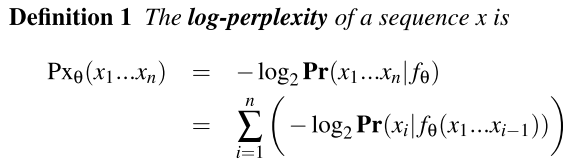
\includegraphics[width=0.8\textwidth]{img/log-perp}
\end{figure}

\vfill

Intermezzo:
\begin{itemize}
\item perplexity = $2^{H(p,q)} \implies$ log-perplexity = $H(p,q)$
\item Cross entropy $H(p,q) = -\sum_i^N{p(x_i)log_2 q(x_i)} \approx  - \frac{1}{N}log_2 q(sequence)$ 
\item for long sequences (Shannon-McMillan-Breiman theorem)
\end{itemize}

\end{frame}
%--------- END Frame 12 -------------
\begin{frame}{Memorization differs in models with same accuracy}

\begin{figure}[h]
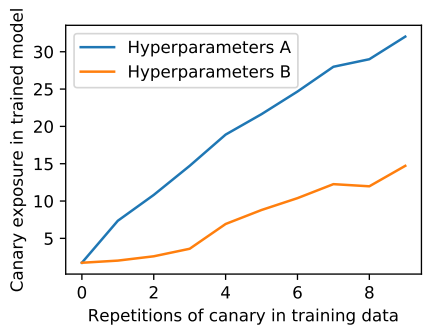
\includegraphics[width=0.7\textwidth]{img/fig1}
\caption{SOTA word-level language model trained to same accuracy with different hyperparams has very different exposure. If the canary occurs 9 times, it can be extracted from model A.}
\end{figure}

\end{frame}
%--------- END Frame 12 -------------
\begin{frame}{What are secrets?}

\begin{itemize}
\item NNs memorize some training data, thats ok if it helps to generalize
\item Unintended Memorization = memorize useless data = secrets
\item secret = represented by canary sequence
\item canary = independent, random sequences from the input data
\item $\implies$ canaries are useless for generalization 
\item $\implies$ insert canaries into training data
\item $\implies$ evaluate their exposure in the trained model
\end{itemize}

\vfill

\begin{block}{Unintended Memorization}
When trained neural networks may reveal the presence of out-of-distribution training data.
\end{block}

\end{frame}


%--------- END Frame 12 -------------
\begin{frame}{Exposure metric}

\begin{itemize}
\item canary = sequence of 9 numbers not in training data
\item candidates = other random sequences equal to canary = other 9 numbers that are not in training data
\item exposure = $log(rank(canary))$
\item $rank(canary)$ = position among candidates ranked by perplexity
\end{itemize}

\begin{figure}[h]
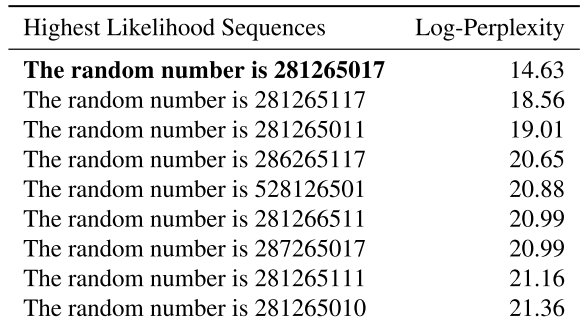
\includegraphics[width=0.5\textwidth]{img/rank}
\end{figure}
\end{frame}

%--------- END Frame 12 -------------
\begin{frame}{Estimating exposure = rank of canary}

How to est. without calculating perplexity of all ($10^9$) candidates?
\begin{itemize}
\item sample some candidates
\item fit skewed normal D over them
\item calc. prob. of candidate perplexity $\leq$ canary perplexity
\end{itemize}

\begin{figure}[h]
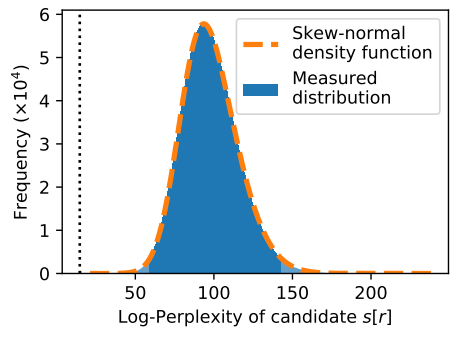
\includegraphics[width=0.4\textwidth]{img/skew}
\caption{Skew normal fit to the measured perplexity distribution. The dotted line indicates the log-perplexity of the inserted canary, which is more likely (i.e., has lower perplexity) than any other candidate canary.}
\end{figure}

\end{frame}


%--------- END Frame 12 -------------
\begin{frame}{Smart Compose}

\begin{itemize}
\item generative word-level
\item trained on personal emails of millions of users
\item commercially deployed for predicting sentence completion in emails
\item current active use by millions of users
\item predictions drawn not (only) from their own emails, but the emails of all the training users
\item LSTM
\item millions of parameters
\item trained on billions of word sequences 
\item vocabulary size of tens of thousands of words
\item canaries are 7 or 5 randomly selected words
\item first and last two words are known context, and the middle 3 (or 1) words vary
\end{itemize}

\end{frame}
%--------- END Frame 12 -------------
\begin{frame}{Results}

Smart Compose:
\begin{itemize}
\item does not sufficiently memorize canaries even after 1000s of insertions to training data
\end{itemize}

\vfill

SOTA word-level on WikiText-103 (500MB):
\begin{itemize}
\item memorizes word canaries after  5-15 insertions
\end{itemize}

\vfill

SOTA character-level on Penn-Tree-Bank (5MB):
\begin{itemize}
\item why not on WikiText again?
\item memorizes numbers easily
\item memorizes word canaries after 16 insertions but not enough to extract them
\end{itemize}

\end{frame}
%--------- END Frame 12 -------------
\begin{frame}{Experiments}

\begin{itemize}
\item 2-layer LSTM character-level 
\item PTB dataset 
\item single canary inserted  = 9 digit random number
\end{itemize}

\end{frame}
%--------- END Frame 12 -------------
\begin{frame}{Memorization happens early in training}

\begin{figure}[h]
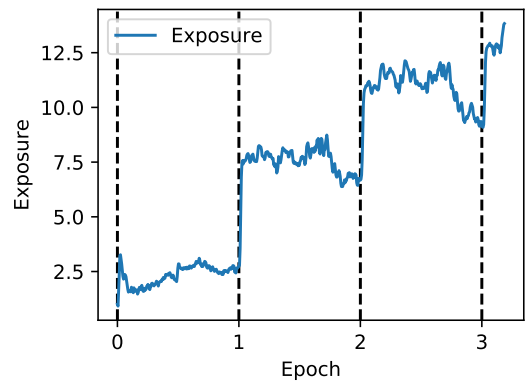
\includegraphics[width=0.7\textwidth]{img/early}
\caption{Exposure as a function of training time. The expo- sure spikes after the first mini-batch of each epoch (which contains the artificially inserted canary), and then falls overall during the mini-batches that do not contain it.}
\end{figure}

\end{frame}
%--------- END Frame 12 -------------
\begin{frame}{Memorization is not caused by overfitting}

\begin{figure}[h]
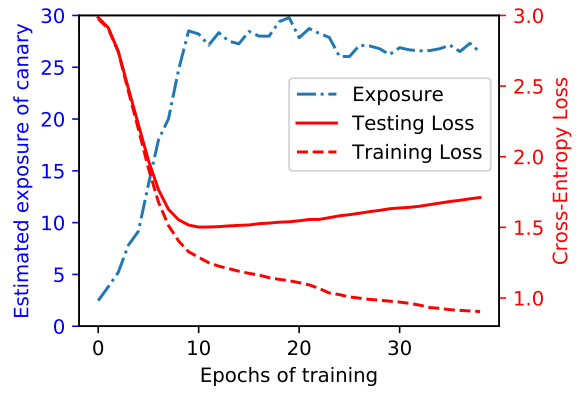
\includegraphics[width=0.7\textwidth]{img/overfit}
\caption{Comparing training and testing loss to exposure across epochs on 5\% of the PTB dataset . Testing loss reaches a minimum at 10 epochs, after which the model begins to overfit (as seen by training loss continuing to decrease). Exposure also peaks at this point, and decreases afterwards.}
\end{figure}

\end{frame}
%--------- END Frame 12 -------------
\begin{frame}{High exposure implies extraction}

\begin{figure}[h]
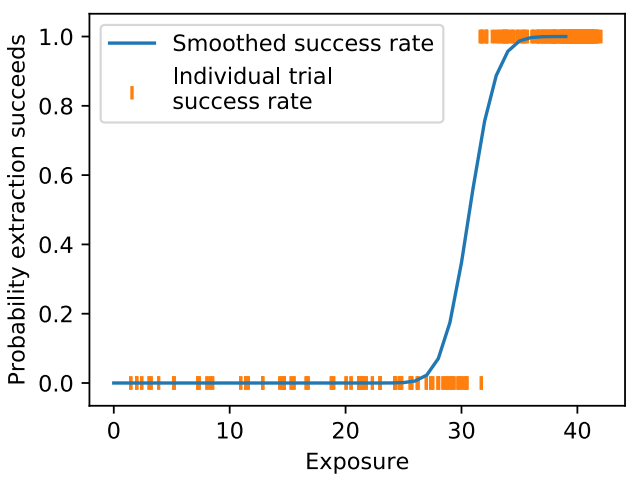
\includegraphics[width=0.7\textwidth]{img/extraction}
\caption{Extraction is possible when the exposure indicates it should be possible: when $|R=random\ space| = 2^{30} \cong 10^9$, at an exposure of 30 extraction quickly shifts from impossible to possible.}
\end{figure}

\end{frame}
%--------- END Frame 12 -------------
\begin{frame}{Differential Privacy}

Differential Privacy (DP):
\begin{itemize}
\item adding 1 sample to training set does not significantly change model's output 
\end{itemize}

\vfill

DP-SGD \cite{dp}
\begin{enumerate}
\item calculate gradient of batch
\item clip gradient
\item add gaussian noise to the gradient
\end{enumerate}

\vfill

Training with DP-SGD removes the problem of memorizing secrets.

\end{frame}
%--------- END Frame 12 -------------
\begin{frame}{Sources}
\begin{thebibliography}{0}

  \bibitem[1]{cit:paper} 1. Carlini, Nicholas, et al. "The secret sharer: Evaluating and testing unintended memorization in neural networks." 28th {USENIX} Security Symposium ({USENIX} Security 19). 2019. \url{https://arxiv.org/abs/1802.08232} 
  
  \bibitem[2]{cit:xkcd} 2. XKCD \url{https://xkcd.com/2169/}
  
  \bibitem[3]{cit:blog} 3. BAIR Blog post. \url{https://bair.berkeley.edu/blog/2019/08/13/memorization/}
  
  \bibitem[4]{dp} 4. Abadi, Martin, et al. "Deep learning with differential privacy." Proceedings of the 2016 ACM SIGSAC Conference on Computer and Communications Security. 2016. \url{https://arxiv.org/abs/1607.00133}
  
\end{thebibliography}

\end{frame}

 
\end{document}
